%----------------------------------------------------------------------
%	Packages and other document configurations
%----------------------------------------------------------------------
%% Page Setup
\documentclass[10pt, final]{report}	
\usepackage[a4paper, margin=2.5cm]{geometry} 

%% Language, input and output options
\usepackage[english]{babel}
\usepackage[T1]{fontenc}
\usepackage[utf8]{inputenc}  % Unicode Characters
%\usepackage{newtxmath,newtxtext} % Times New Roman 
\usepackage[urw-garamond]{mathdesign} % But Garamond is better
\usepackage{hologo}
\usepackage{lettrine}
\usepackage{setspace}

%% Graphics and float packages
\usepackage{rotating} % To rotate a page if nessacary
\usepackage{graphicx} % Required for including pictures
\usepackage{wrapfig} % Allows in-line images
\usepackage{caption}
\usepackage{subcaption}	
\usepackage{float} % Allows putting an [H] to specify exact location 
\graphicspath{{../figures/}} % Directory where pictures are stored
\usepackage{pdflscape}
\usepackage{tikz}

%% Inclusion of other packages
\usepackage[sort&compress,round,semicolon,authoryear]{natbib}
\usepackage{siunitx}
\usepackage{gensymb}
\usepackage{pdfpages}
\usepackage{tabularx}
\usepackage[linguistics]{forest} % To create pretty diagrams
\usepackage{tikz-qtree}
\usetikzlibrary{shapes,arrows}
\usepackage{enumitem}
\usepackage{listings}

%% Configure the TOC and center the TOC, LOF and LOT title
\addtocontents{toc}{~\hfill\textbf{Page}\par}
\usepackage[numbib]{tocbibind}
\usepackage{tocloft}
\renewcommand{\cfttoctitlefont}{\hspace*{\fill}\huge\bfseries}
\renewcommand{\cftaftertoctitle}{\hspace*{\fill}}
\renewcommand{\cftlottitlefont}{\hspace*{\fill}\huge\bfseries}
\renewcommand{\cftafterlottitle}{\hspace*{\fill}}
\renewcommand{\cftloftitlefont}{\hspace*{\fill}\huge\bfseries}
\renewcommand{\cftafterloftitle}{\hspace*{\fill}}

%% Setup titles and sectioning
\usepackage{titlesec}
\titleformat{\chapter}[display]
  {\normalfont\huge\bfseries\centering}
  {\chaptertitlename\ \thechapter}{-5pt}{\huge}
  \titlespacing*{\chapter}{0pt}{-50pt}{10pt}
  
\titlespacing*{\section}
{0pt}{1ex plus 1ex minus .2ex}{1ex plus .2ex}

\titlespacing*{\subsection}
{0pt}{1ex plus 1ex minus .1ex}{1ex plus .1ex}

\titleformat{\paragraph}
	{\normalfont\normalsize\bfseries}{\theparagraph}{1em}{}
	\titlespacing*{\paragraph}
	{0pt}{1ex plus 1ex minus .1ex}{1ex plus .1ex}

%% Modify links
\usepackage[hyphens]{url}
\usepackage[colorlinks=true,urlcolor=black,citecolor=black,linkcolor=black,bookmarks=true,pagebackref]{hyperref} % colored citations
\renewcommand{\backrefxxx}[3]{%
  (\hyperlink{page.#1}{$\uparrow$#1})} % This is to add backref^
\usepackage[hyphenbreaks]{breakurl}
\usepackage{bookmark}
\bookmarksetup{numbered,open}

%% Figure out the glossary
\usepackage[toc]{glossaries}
\newglossary{abbreviation}{aot}{ata}{List of Abbreviations}
\loadglsentries[abbreviation]{glossaries}
\makeglossaries

%% Setup tikz, bookmarks, colors
\colorlet{linecol}{black!75}
\usetikzlibrary{arrows.meta}
\tikzset{
  my rounded corners/.append style={rounded corners=2pt},
}

%% Change lengths and minimize whitespace
\setlength{\parindent}{0pt}
\setlength{\parskip}{0.5em plus 0.2em minus 0.2em}
\linespread{1.2} % Line spacing\frac{(\overline{w'c'})
\setcounter{secnumdepth}{0} % only number chapters
\setcounter{tocdepth}{1}
\setlength{\cftbeforetoctitleskip}{0pt}
\setlength{\cftbeforeloftitleskip}{0pt}
\setlength{\cftbeforelottitleskip}{0pt}
\setlength\cftparskip{0pt}
\setlength\cftbeforechapskip{0pt}

%% Pdf Metadata
\hypersetup{
    pdftitle={Latex is for cool kids},
    pdfsubject={Not Computer Science},
    pdfauthor={Piet Pompies},
    pdfkeywords={Linux, LaTeX, Debian, Github}
}

% document begin
\begin{document}

%--------------------------------------------------------------------
%	Title Page
%--------------------------------------------------------------------
\pagenumbering{Roman}
\begin{titlepage}
\thispagestyle{empty}
\centering
\vspace*{3em}
\linespread{2}\selectfont
{\LARGE\bfseries 
The Impact of Focus Structure on Pronoun Resolution Among Non-native English and French Speakers}

\vspace{5em}
\linespread{1}\selectfont
\LARGE
Zhou Da

\bigskip
\Large
Under the Supervision of Xu Xiaodong

\vspace{5em}
\linespread{1.2}\selectfont
In Partial Fulfillment of \\
the Requirement for Bachelor's Degree\\
Submitted to\\
School of Foreign Languages and Cultures\\
Nanjing Normal University\\

\vspace{5em}
May, 2018

\end{titlepage}
%\newpage\mbox{}\thispagestyle{empty}\newpage
\thispagestyle{empty}

%--------------------------------------------------------------------
%	Declaration
%--------------------------------------------------------------------
% ******************************* Thesis Declaration ***************************

\begin{declaration}

I hereby declare that except where specific reference is made to the work of 
others, the contents of this dissertation are original and have not been 
submitted in whole or in part for consideration for any other degree or 
qualification in this, or any other university. This dissertation is my own 
work and contains nothing which is the outcome of work done in collaboration 
with others, except as specified in the text and Acknowledgements. This 
dissertation contains fewer than 65,000 words including appendices, 
bibliography, footnotes, tables and equations and has fewer than 150 figures.

% Author and date will be inserted automatically from thesis.tex \author \degreedate

\end{declaration}


\thispagestyle{empty}
\newpage

%--------------------------------------------------------------------
%	Abstract
%--------------------------------------------------------------------
% Abstract
\clearpage
\thispagestyle{plain}
\phantomsection
\addcontentsline{toc}{chapter}{Abstract}

\centerline{\zihao{3}\bfseries Abstract}

\linespread{1.4}\zihao{-4}
\bigskip

This thesis explores the relationship between focus structure and pronoun resolution among non-native speakers of English and French. Firstly we reviewed the existing literature on the mechanism of focus effect and pronoun resolution. Then through a self-paced reading test, we find that focus, in the form of cleft structure does not necessarily increase the salience of a informational unit, thus may not in some cases make it a preferred antecedent for pronoun resolution. This result is line with previous researches on this topic. In our experiment, We also find that focused subject in French and focused object in English are processed faster, but focused subjects in both languages leads to longer response time of anaphora. Furthermore, our research also shows that the congruence between anaphora and focus does not make the latter more accessible. In this regard, we argue that the problem of whether there is subject or object preference in English and French is more complicated than the results of current studies.

\bigskip
\noindent\textbf{\zihao{4} Keywords:} 
focus effect, pronoun resolution, self-paced reading, English, French


\newpage

%--------------------------------------------------------------------
%	Dedication
%--------------------------------------------------------------------
% ******************************* Thesis Dedidcation ********************************

\begin{dedication} 

To Ash \textit{et al.}

\end{dedication}

\newpage

%--------------------------------------------------------------------
%	Preface
%--------------------------------------------------------------------
\chapter*{Preface}
\setheader{Preface}

Preface\ldots

\begin{flushright}
{\makeatletter\itshape
    \@author \\
    Delft, January 2013
\makeatother}
\end{flushright}


\newpage

%--------------------------------------------------------------------
%	Table of Contents
%--------------------------------------------------------------------
\pagenumbering{Roman}
\tableofcontents % Include a table of contents
%\addtocontents{toc}{~\hfill\textbf{Page}\par}
\newpage % Begins the LoF on a new page  

%--------------------------------------------------------------------
%	List of Figures
%--------------------------------------------------------------------
\listoffigures
\addtocontents{lof}{~\hfill\textbf{Page}\par}
\newpage

%--------------------------------------------------------------------
%	List of Tabels
%--------------------------------------------------------------------
\listoftables
\addtocontents{lot}{~\hfill\textbf{Page}\par}

%--------------------------------------------------------------------
%	List of Abbreviations
%--------------------------------------------------------------------
\printglossaries
\newpage

%--------------------------------------------------------------------
%	Chapter 1: Introduction and Litrature study
%--------------------------------------------------------------------
%----------------------------------------------------------------------------------------
%	INTRODUCTION & BACKGROUND
%----------------------------------------------------------------------------------------
\pagenumbering{arabic}
\setcounter{section}{0}
\renewcommand*{\theHsection}{chX.\the\value{section}}

\chapter{Introduction and literature review}
\label{Introduction and literature review}
\lipsum

\section{This is a section}
\lipsum

\subsection{This is a subsection}
\lipsum

\subsubsection{This is a subsubsection}
\lipsum
 

%--------------------------------------------------------------------
%	Chapter 2: Aims, Objectives and Layout
%--------------------------------------------------------------------
%----------------------------------------------------------------------------------------
%	Aims, Objectives and Layout
%----------------------------------------------------------------------------------------

\section{Aims and objectives}

Bla Bla 

\begin{enumerate}
\item bullet points
\item are done 
\item like this 
\end{enumerate}

\section{Study design}
\lipsum

\newpage

%--------------------------------------------------------------------
%	Chapter 3: Study Area, Data & Methods
%--------------------------------------------------------------------
%----------------------------------------------------------------------------------------
%	Study Area, Data and Methods
%----------------------------------------------------------------------------------------
\chapter{Data and methods}
\lipsum

\newpage

%--------------------------------------------------------------------
%	Chapter 4: 
%--------------------------------------------------------------------
%--------------------------------------------------------------------------
% The of the results <- use % to comment
%--------------------------------------------------------------------------
\chapter{\LaTeX is so awesome}
\lipsum

\newpage

%--------------------------------------------------------------------
%	Chapter 5: 
%--------------------------------------------------------------------
%--------------------------------------------------------
% Another Chapter 
%--------------------------------------------------------
\chapter{\LaTeX is for professionals}
\lipsum

\newpage

%--------------------------------------------------------------------
%	Chapter 6: 
%--------------------------------------------------------------------
%------------------------------------------------------------------
% The last chapter
%------------------------------------------------------------------

\chapter{Support \LaTeX}
\lipsum

\section{This is another section}
\lipsum

\subsection{This is another subsection}
\lipsum

\paragraph{This a paragraph}
\lipsum

\newpage

%--------------------------------------------------------------------
%	Conclusion
%--------------------------------------------------------------------
% !Mode:: "TeX:UTF-8" 
\begin{conclusions}

学位论文的结论作为论文正文的最后一章单独排写,但不加章标题序号。

结论应是作者在学位论文研究过程中所取得的创新性成果的概要总结,不能与摘要混为一谈。博士学位论文结论应包括论文的主要结果、创新点、展望三部分,在结论中应概括论文的核心观点,明确、客观地指出本研究内容的创新性成果(含新见解、新观点、方法创新、技术创新、理论创新),并指出今后进一步在本研究方向进行研究工作的展望与设想。对所取得的创新性成果应注意从定性和定量两方面给出科学、准确的评价,分(1)、(2)、(3)…条列出,宜用“提出了”、“建立了”等词叙述。

\end{conclusions}

\newpage

%--------------------------------------------------------------------
%	Bibliography
%--------------------------------------------------------------------
\linespread{0.9} \normalsize
\bibliographystyle{agsm} % Bibliography style
\renewcommand{\bibpreamble}{$\uparrow$ refers back to in text citations}
\bibliography{../bibliography/master}
\label{sec:bib}

%--------------------------------------------------------------------
%   Appendix
%--------------------------------------------------------------------
\newpage
\linespread{1.2} \normalsize
%%%%%%%%%%%%%%%%%%%%% appendix.tex %%%%%%%%%%%%%%%%%%%%%%%%%%%%%%%%%
%
% sample appendix
%
% Use this file as a template for your own input.
%
%%%%%%%%%%%%%%%%%%%%%%%% Springer-Verlag %%%%%%%%%%%%%%%%%%%%%%%%%%

\chapter{Chapter Heading}
\label{introA} % Always give a unique label
% use \chaptermark{}
% to alter or adjust the chapter heading in the running head

Use the template \emph{appendix.tex} together with the Springer document class SVMono (monograph-type books) or SVMult (edited books) to style appendix of your book in the Springer layout.


\section{Section Heading}
\label{sec:A1}
% Always give a unique label
% and use \ref{<label>} for cross-references
% and \cite{<label>} for bibliographic references
% use \sectionmark{}
% to alter or adjust the section heading in the running head
Instead of simply listing headings of different levels we recommend to let every heading be followed by at least a short passage of text. Further on please use the \LaTeX\ automatism for all your cross-references and citations.


\subsection{Subsection Heading}
\label{sec:A2}
Instead of simply listing headings of different levels we recommend to let every heading be followed by at least a short passage of text. Further on please use the \LaTeX\ automatism for all your cross-references and citations as has already been described in Sect.~\ref{sec:A1}.

For multiline equations we recommend to use the \verb|eqnarray| environment.
\begin{eqnarray}
\vec{a}\times\vec{b}=\vec{c} \nonumber\\
\vec{a}\times\vec{b}=\vec{c}
\label{eq:A01}
\end{eqnarray}

\subsubsection{Subsubsection Heading}
Instead of simply listing headings of different levels we recommend to let every heading be followed by at least a short passage of text. Further on please use the \LaTeX\ automatism for all your cross-references and citations as has already been described in Sect.~\ref{sec:A2}.

Please note that the first line of text that follows a heading is not indented, whereas the first lines of all subsequent paragraphs are.

% For figures use
%
\begin{figure}[t]
\sidecaption[t]
% Use the relevant command for your figure-insertion program
% to insert the figure file.
% For example, with the graphicx style use
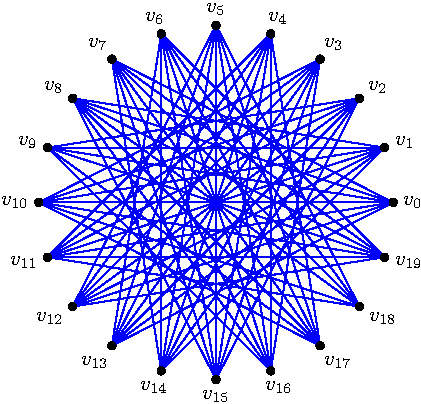
\includegraphics[scale=.65]{figure}
%
% If no graphics program available, insert a blank space i.e. use
%\picplace{5cm}{2cm} % Give the correct figure height and width in cm
%
\caption{Please write your figure caption here}
\label{fig:A1}       % Give a unique label
\end{figure}

% For tables use
%
\begin{table}
\caption{Please write your table caption here}
\label{tab:A1}       % Give a unique label
%
% Follow this input for your own table layout
%
\begin{tabular}{p{2cm}p{2.4cm}p{2cm}p{4.9cm}}
\hline\noalign{\smallskip}
Classes & Subclass & Length & Action Mechanism  \\
\noalign{\smallskip}\hline\noalign{\smallskip}
Translation & mRNA$^a$  & 22 (19--25) & Translation repression, mRNA cleavage\\
Translation & mRNA cleavage & 21 & mRNA cleavage\\
Translation & mRNA  & 21--22 & mRNA cleavage\\
Translation & mRNA  & 24--26 & Histone and DNA Modification\\
\noalign{\smallskip}\hline\noalign{\smallskip}
\end{tabular}
$^a$ Table foot note (with superscript)
\end{table}
%


%--------------------------------------------------------------------
%--------------------------------------------------------------------

\end{document}
